\chapter{Аналитическая часть}

\section{Анализ предметной области}

Спортивным залом зачастую называется целый спортивный комплекс, имеющий множество специализированных пространств 
для проведения тренировок. Такое предприятие организовывает множество людей, например тренеров, клиентов, 
администраторов. Необходимо регулировать назначение тренировок, запись клиентов, штат администраторов и тренеров,
ведение персональных статистик, составление расписания залов и спортивных мероприятий.

\section{Сравнительный анализ существующих конкурентов}

Для анализа были выбраны популярные приложения с высокими рейтингами, такие как:

\begin{itemize}[label=—]
	\item 1С:Фитнес-клуб \cite{1cfitness};
	\item Mobifitness \cite{mobifitness};
	\item FitBase \cite{fitbase};
	\item Sport Priority \cite{sportpriority}.
\end{itemize}

При анализе будут учитываться следующие критерии:

\begin{enumerate}
	\item управление персоналом;
	\item учёт клиентов;
	\item управление графиком персонала;
	\item возможность ведения клиентом персональной статистики;
	\item управление спортивными пространствами;
	\item управление тренировками.
\end{enumerate}

В таблице \ref{tab:anal} приведены результаты анализа.

\begin{table}[H]
	\centering
	\caption{Результаты анализа существующих конкурентов}
	\begin{tabular}{|c|p{3cm}|p{3cm}|p{2cm}|p{3cm}|}
	\hline
	Номер критерия & 1С:Фитнес-клуб & Mobifitness & FitBase & Sport Priority \\
	\hline
	1 & + & + & + & + \\
	\hline
	2 & + & + & + & + \\
	\hline
	3 & + & - & - & + \\
	\hline
	4 & - & + & - & - \\
	\hline
	5 & + & + & - & - \\
	\hline
	6 & + & + & + & + \\
	\hline
	\end{tabular}
	\label{tab:anal}
\end{table}

\section{Требования к разрабатываемой базе данных и приложению}

База данных должна включать в себя данные о клиентах, администраторах, тренерах, тренировках,
спортивных пространствах.

Приложение должно позволять выполнять следующие операции:

\begin{enumerate}
	\item авторизовываться как клиент, тренер, администратор;
	\item управлять персональными статистиками клиентов;
	\item управлять расписаниями спортивных пространств;
	\item управлять персоналом и клиентами;
	\item управлять тренерскими специализациями;
	\item управлять рабочими часами тренера;
	\item управлять групповыми мероприятими и тренировками;
	\item управлять персональными тренировками.
\end{enumerate}

\section{Формализация и описание информации, подлежащей хранению в проектируемой базе данных}

В таблице \ref{tab:formaldb} описана информация, подлежащая хранению в базе данных.

\begin{table}[H]
	\centering
	\caption{Категории данных в базе данных и их свойства}
	\begin{tabular}{|p{6cm}|p{10cm}|}
	\hline
	Категория & Информация \\
	\hline
	Тренер & идентификатор, имя, фамилия, логин, пароль, статус(уволен, работает) \\
	\hline
    Вид тренерской специализации & идентификатор, название, идентификатор зала проведения \\
	\hline
	Связь тренеров и видов специализаций & идентификатор, идентификатор тренера, идентификатор специализации \\
	\hline
	Рабочие часы тренера & идентификатор, идентификатор тренера, дата, время начала, время окончания \\
	\hline
	Клиент & идентификатор, имя, фамилия, логин, пароль, статус(посещает зал, перестал ходить) \\
	\hline
	Виды персональных статистик & идентификатор, название, единица измерения \\
	\hline
	Связь статистик клиентов & идентификатор, идентификатор клиента, идентификатор статистики, значение, дата \\
	\hline
	Администратор & идентификатор, имя, фамилия, логин, пароль, статус(уволен, работает) \\
	\hline
	Групповое мероприятие & идентификатор, название, идентификатор назначившего администратора, идентификатор тренера, идентификатор спортивного пространства, вместимость, продолжительность, дата и время \\
	\hline
	Спортивное пространство & идентификатор, название \\
	\hline
	Расписание работы спортивного пространства & идентификатор, идентификатор спортивного пространства, дата, время начала, время окончания \\
	\hline
	Записи на мероприятия & идентификатор, идентификатор клиента, идентификатор группового мероприятия \\
	\hline
	Индивидуальные тренировки & идентификатор, идентификатор тренера, идентификатор клиента, идентификатор спортивного пространства, дата и время, продолжительность, дополнительная информация \\
	\hline
	\end{tabular}
	\label{tab:formaldb}
\end{table}

\section{Анализ существующих баз данных на основе формализации данных}

Существует три основных типа баз данных: 
\begin{enumerate}
	\item дореляционные;
	\item реляционные;
	\item постреляционные.
\end{enumerate}

\subsection{Дореляционные базы данных}

Дореляционные базы данных \cite{DBModels} хранят записи в виде связей родитель-ребёнок. Основными моделями таких 
баз являются иерархическая и сетевая. Основное отличие между ними заключается в том, что иерархическая модель не поддерживает 
отношение многие-ко-многим, так как каждый ребёнок может иметь только одного родителя. 
В свою очередь в сетевой моделе у каждого ребёнка может быть несколько родителей.

Основными недостатками дореляционных баз данных являются избыточность данных и сложность выполнения запросов.
Масштабируемость затруднена из-за сложности изменения структуры, гибкость крайне ограничена. Целостность данных поддерживается, 
но за счёт жёсткой структуры связей.

\subsection{Реляционные базы данных}

В реляционных базах данных данные хранятся в виде двумерных таблиц. Связь между ними обеспечивается общими столбцами, такими как 
идентификаторы. Таблицная архитектура реализует эффективный способ хранения структурированной информации.

Они обеспечивают гибкий и масштабируемый способ хранения и управления большими объемами данных, 
гарантируя при этом целостность и непротиворечивость данных с помощью ограничений.

\subsection{Постреляционные базы данных}

Такие базы данных позволяют удобно хранить неструктурированные данные, поддерживая логические связи между ними. 
Постреляционные базы отлично подходят для данных с изменчивой структурой и высоконагруженных приложений.
Недостатком является сложность обеспечения целостности данных.

Отличаются высокой гибкостью структуры, хорошей горизонтальной масштабируемостью. 
Сложность запросов варьируется в зависимости от конкретной реализации. 

\subsection{Вывод}

Для реализации поставленной задачи была выбрана реляционная модель, так как она лучше всего подходит для хранения 
структурированной информации, обеспечивая баланс между целостностью данных, гибкостью запросов и возможностями масштабирования.

\section{Формализация и описание пользователей проектируемого приложения к базе данных}

Гость, или неавторизованный пользователь может войти как клиент, тренер, или администратор.

Администратор может:

\begin{enumerate}
	\item управлять видами индивидуальных статистик клиентов;
	\item управлять расписанием работы спортивных пространств;
	\item управлять клиентами, тренерами, и другими администраторами;
	\item управлять специализациями тренеров;
	\item управлять рабочими часами тренеров;
	\item управлять групповыми мероприятиями;
	\item просматривать проводимые тренировки тренеров.
\end{enumerate}

Тренер может:

\begin{enumerate}
	\item управлять своими рабочими часами;
	\item управлять персональными тренировками;
	\item просматривать предстоящие тренировки и мероприятия;
	\item просматривать доступные залы для проведения тренировок в зависимости от его специализаций.
\end{enumerate}

Клиент может:

\begin{enumerate}
	\item управлять персональной статистикой;
	\item просматривать доступные мероприятия;
	\item управлять записями на мероприятия и тренировки;
	\item отменять персональные тренировки.
\end{enumerate}

\section{Диаграмма прецедентов}

На рисунке \ref{fig:graph} представлена диаграмма прецедентов.

\begin{figure}[H]
	\centering
	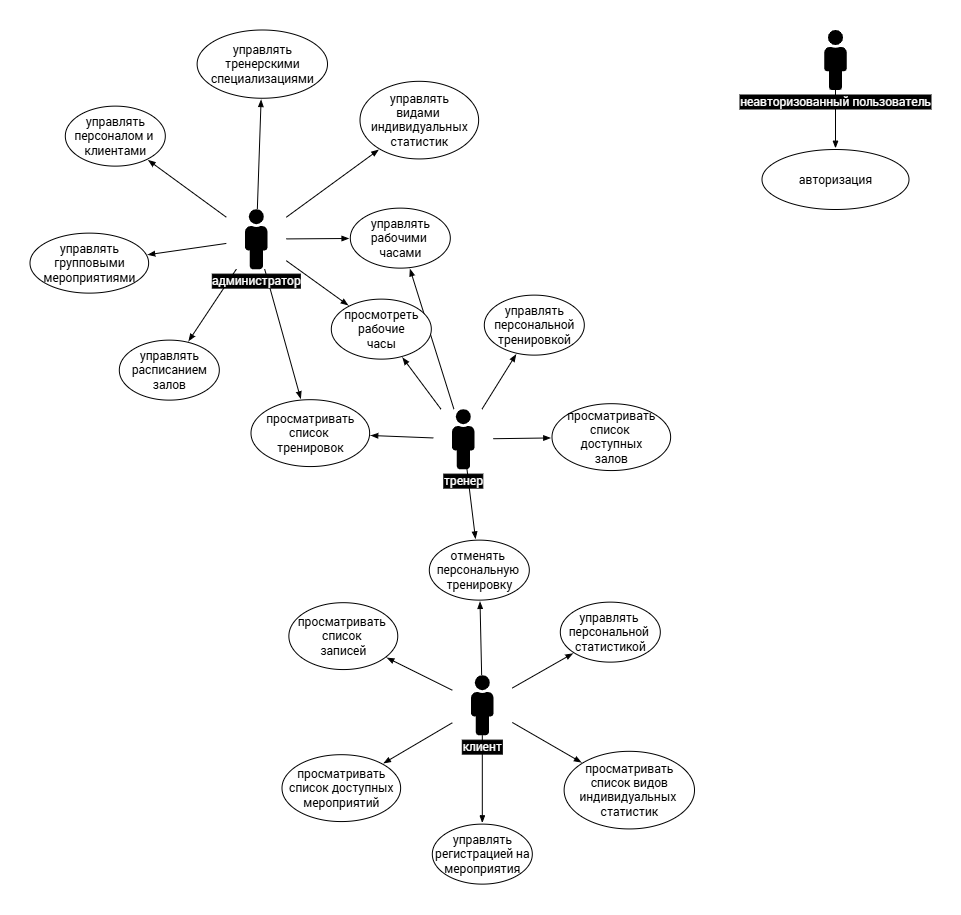
\includegraphics[width=1\textwidth]{img/usecase.png}
	\caption{Диаграмма прецедентов}
	\label{fig:graph}
\end{figure}

\section{Формализация задачи}

На основании проведённого анализа предметной области, требований к разрабатываемой базе данных и приложению,
сравнительного анализа предметной области, формализация задачи проектирования базы данных и приложения для спортивного 
зала звучит следующим образом:

Требуется создать информационную систему спортивного зала с использованием реляционной базы данных для управления:

\begin{enumerate}
	\item клиентами;
	\item тренерами;
	\item администраторами;
	\item графиком работы персонала;
	\item спортивными пространствами;
	\item групповыми и индивидуальными тренировками;
	\item персональными клиентскими статистиками.
\end{enumerate}

На рисунке \ref{fig:er_diagram} представлена диаграмма сущность-связь проектируемой базы данных.

\begin{figure}[H]
    \centering
    \includegraphics[height=0.65\textheight, angle=90]{img/er.pdf}
    \caption{Диаграмма сущность-связь проектируемой базы данных}
    \label{fig:er_diagram}
\end{figure}